\subsection{Effect of Preserving the Physical State}
\label{sec:controlled-ablation}
\begin{table*}[t]\centering\scriptsize
\caption{Controlled amplitude-score and physical-state-carry ablation. Same five-model bank and publication rules. All 18 continuous parents (108 events) are retained. Normal controls comprise three 600-s records with 588 s evaluated exposure each (1,764 s total; startup excluded). Delay is conditional on emitted matched diagnoses and must be read with the no-timely-diagnosis count.}
\label{tab:a01}
\begin{tabular}{lrrrrrr}\toprule
Procedure & Timely & Extras & Normal FA & False restorations & No timely & Delay (s)\\\midrule
Marginal + carry & 108/108 & 1 & 0/1,764 s & 1 & 0/108 & 0.267\\
Profile + carry & 108/108 & 1 & 0/1,764 s & 1 & 0/108 & 0.267\\
Marginal + reset & 75/108 & 166 & 0/1,764 s & 130 & 33/108 & 0.337\\
Profile + reset & 75/108 & 166 & 0/1,764 s & 130 & 33/108 & 0.337\\
\bottomrule\end{tabular}\end{table*}

\begin{figure*}[t]\centering
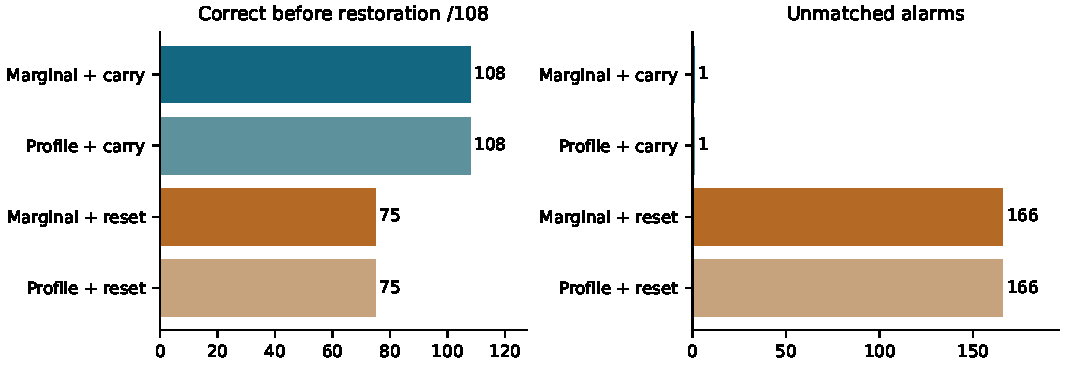
\includegraphics[width=.92\textwidth]{figures/generated/ablation_a01.pdf}
\caption{Severity-scoring and state-carry study on identical observations and five-model banks. The 108 interventions belong to 18 continuous trajectories. Thresholds are fixed, so the alarm rate may differ between arms.}\label{fig:a01}\end{figure*}
The nominal bank and the continuous GLR both carry physical state.
Their primary comparison therefore cannot identify the effect of resetting
it. In the fixed-threshold component study, resetting only the physical
coordinates reduced timely attribution from 108/108 to 75/108 and increased
unmatched alarms from 1 to 166 (Table~\ref{tab:a01} and Fig.~\ref{fig:a01}).
Marginal and profile severity scores gave the same outcomes within each
state treatment. The simulation itself evolves continuously in all arms.

\begin{figure}[t]\centering
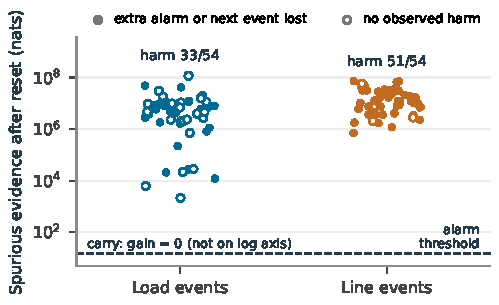
\includegraphics[width=\columnwidth]{figures/generated/theory_reset_cost.pdf}
\caption{Retrospective profiled energy gain after a state reset, \eqref{eq:reset-bias}, for the 108 interventions of the controlled study. Filled: an extra alarm in the following gap or a lost timely attribution of the next intervention; open: neither. The dashed line is the idealized score reference, not the publication threshold. Under matched noise-free continuation, carrying the state gives no positive gain over the null.}
\label{fig:theory-reset}\end{figure}

Fig.~\ref{fig:theory-reset} compares this outcome with the retrospective reset diagnostic. The
profiled energy gain exceeds $\lambda^\star$ after every intervention, by at
least two and up to seven orders of magnitude, and the reset arm is harmed
after \RevResetHarm{} of the \RevResetEvents{} interventions: an extra alarm
in the following gap or a lost timely attribution of the next one. Harm
occurs after \RevResetHarmLine{} line events and
\RevResetHarmLoad{} load events. The bus-31 events carry the smallest
profiled gain and are harmed after three of seven. The diagnostic shows
that reset leaves a residual that event candidates can explain. Its
magnitude alone does not determine the observed outcome: episode handling
and publication rules also matter. These are within-simulator contrasts at the
original thresholds; the two scores are compared at equal thresholds, not
at equal alarm rates.
